\section{External Evaluation and Failure Analysis}
\label{sec:external}

\paragraph{Setup.} The unchanged pipeline analysed the UCI-498 incident
log~\cite{amaral2018uci498}, a real ServiceNow event log of one organization's IT
service desk, with each final assignment group of sufficient size treated as an
entity: 50 groups, 22,604 of 24,918
incidents, 47,420 investigation-step proxies derived from work-state events
and 19,656 escalation proxies derived from reassignments. The only outcome
available is the final SLA flag. SLA labels were loaded only after SAT-SA's ranking
existed and never entered a submission. \emph{This is IT incident data, not SOC data};
it is, however, the log on which prior work demonstrated incident-management
compliance assessment~\cite{palma2024eurova} and modelled SLA
attainment~\cite{swain2022sla}.

\paragraph{Feasibility.} All 134,888 submitted rows were accepted
(0 rejected) and every group's analysis completed, with a median
of 9\,s per group.

\paragraph{Negative result.} SAT-SA's risk $R_e$ was not associated with the SLA-miss
rate: Spearman $\rho=\ensuremath{-}0.11$, 95\% bootstrap \ensuremath{-}0.42 to
0.21 (Table~\ref{tab:external}, Fig.~\ref{fig:external}). Slowest median
resolution reached $\rho=0.94$ (0.86 to
0.97), as expected for a timeliness outcome; reassignment rate
reached 0.37. Among the 12 groups in the top SLA-miss
quartile, SAT-SA's precision@10\% was 0.40 (random 0.25,
slowest resolution 1.00), and it needed to review 50
groups to find all of them (slowest resolution 24).

\begin{table}[t]
\caption{UCI-498 IT incident log (X02b, X03): Spearman association of group scores
with the SLA-miss rate over 50 assignment groups of one organization
(95\% seeded bootstrap intervals). Not SOC data.}
\label{tab:external}
\centering
\scriptsize
\begin{tabular}{@{}L{6.2cm}rr@{}}
\toprule
Group score & Spearman $\rho$ & 95\% interval \\
\midrule
SAT-SA risk $R_e$ & \ensuremath{-}0.11 & \ensuremath{-}0.42 to 0.21 \\
Incident volume & \ensuremath{-}0.15 & \ensuremath{-}0.42 to 0.16 \\
Reassignment rate & 0.37 & 0.08 to 0.60 \\
Slowest median resolution (upper reference) & 0.94 & 0.86 to 0.97 \\
\midrule
Execution-gap dimension of $R_e$ (X03) & \ensuremath{-}0.41 & \ensuremath{-}0.66 to \ensuremath{-}0.11 \\
Fast-closure prevalence (X03) & \ensuremath{-}0.70 & \ensuremath{-}0.82 to \ensuremath{-}0.52 \\
\bottomrule
\end{tabular}
\end{table}


\begin{figure}[t]
\centering
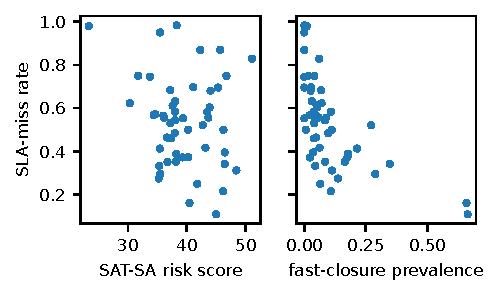
\includegraphics[width=0.78\linewidth]{figures/fig-external.pdf}
\caption{UCI-498 IT incident log (not SOC data): SAT-SA risk (left) and fast-closure
prevalence (right) against the SLA-miss rate; one point per assignment group
(50 groups; X02b, X03).}
\label{fig:external}
\end{figure}

\paragraph{Failure analysis.} A diagnostic analysis (X03) on the same data changed no
detector, threshold or weight. It attributes the result to four causes.
\emph{(i) Construct mismatch (primary).} On a service desk, fast resolution is the
goal: the prevalence of fast closures was \emph{negatively} associated with SLA misses
($\rho=\ensuremath{-}0.70$, \ensuremath{-}0.82 to \ensuremath{-}0.52). SAT-SA treats
fast closure of a security alert as possible skipped investigation, so its execution-gap
dimension, which this signal drives, ran opposite to the outcome
($\rho=\ensuremath{-}0.41$, \ensuremath{-}0.66 to \ensuremath{-}0.11). SLA
timeliness and supervisory execution quality are different constructs, and here they
move in opposite directions. \emph{(ii) Detector saturation.} 4 detector
families fired for every group although their input conditions varied widely---cases
without any step 1.7\% to 78.4\% of cases, medium-or-higher alerts
with fewer than two steps 5.2\% to 85.9\%. Existence rules
cannot discriminate submissions with thousands of tickets, and Eq.~\eqref{eq:risk}
adds near-constant amounts for them because it ignores prevalence; risk still took
49 distinct values and was unrelated to volume
($\rho=0.02$). \emph{(iii) Missing supervisory dimensions.}
3 of the 7 risk dimensions had no input data;
investigation steps and escalations are proxies (state changes and reassignments), and
monitoring coverage is unavailable. \emph{(iv) A minor adapter artifact.} The log has
no step notes; the adapter submits empty notes, which satisfy a repeated-investigation
rule in 39 groups. The analysis found no temporal or label defect: only
3 of 7,907 SLA misses occurred while another group held the
ticket, and reassigned incidents missed more often (53.8\% versus
21.5\%), consistent with the positive reassignment association.

\paragraph{Decision.} No risk-model change was made. Changing detectors or weights to
raise the correlation with SLA misses would optimize SAT-SA toward a timeliness
construct it does not claim to measure, using the evaluation data for tuning. We
therefore read X02b and X03 as \emph{feasibility and construct-validity evidence}, not
as external validation of effectiveness: on data whose outcome measures a different
construct and that lacks investigation, escalation and coverage semantics, SAT-SA's
supervisory signals did not transfer.
